\chapter{Implementation}

\todo[inline]{Game workings}
\todo[inline]{Reducers}
\todo{When remove card from game, all references to it are also removed}

\section{Tools \& Technologies}

\subsection{Node.js}
I decided early on that this application should be easily accessible on a range of devices, particularly the game interface. 
For this reason I built the system as a responsive web-application, running on a node server. 
Node\cite{Node} is an excellent framework for getting sizeable projects up and running very quickly, which I was able to do with this project. 
This is in part due to NPM\cite{npm}, which provides access to countless packages which I was able to use, ranging from Victory\cite{Victory} for visualisations, to Thunk\cite{Thunk} for managing asynchronous side effects.

\subsection{TypeScript}
According to Microsoft who maintain it, `TypeScript is a typed superset of JavaScript that compiles to plain JavaScript'\cite{Typescript}. 
I decided to use TypeScript (TS) to combat some of the problems that can occur when working on a large JavaScript codebase. 
Being statically typed, TS prevents type errors and instantly makes code more navigable and readable. 
This helps both during development and maintenance, which is particularly important if others continue to work on this project.

\subsection{TSLint}
Alongside TypeScript, I set up TSLint\cite{TSLint}, a linter for TypeScript. This was a huge help with development, as TSLint catches issues that can affect the performance of the application. For example, using arrow functions in JSX results in the function being recreated each time the component renders. This can then lead to the component re-rendering due to the shallow comparison of the old and new functions. This can lead to performance issues, which could have been troublesome for the more responsive parts of my software, such as the visualisation page. TSLint also provides general code cleanup features such as organising imports.

\subsubsection{React}
React\cite{React} is a UI library that simplifies the creation of responsive interface components. I knew that I wanted my application to be highly responsive, with each section effectively being split into a single page application. React made this fairly trivial once the structure of the page was settled, as information flows down through components and they are automatically updated.

Using React also encourages the use of inline styles. This makes styles composable, vastly improving reuse of styles and improving maintainability.

\subsubsection{Redux}
Redux \cite{Redux} complements React nicely, by helping to manage state. When using pure React, each component stores it's own state. This can make things confusing as components that should be reflecting information can fall out of sync. Redux encourages moving the state of the whole application into one top-level serializable JS object. This then acts aas a `single source of truth', which takes care of several considerations. Another benefit that I found redux to have is the debugging tools, which take the form of a chrome extension \cite{ReduxDev}. When Redux is correctly used, this tool makes it possible to view and manipulate the application state, and even `time travel' the page to a previous state, such as before a button was clicked. This made debugging very straightforward, particularly for the game logic.

\begin{figure}[!h]
	\centering
	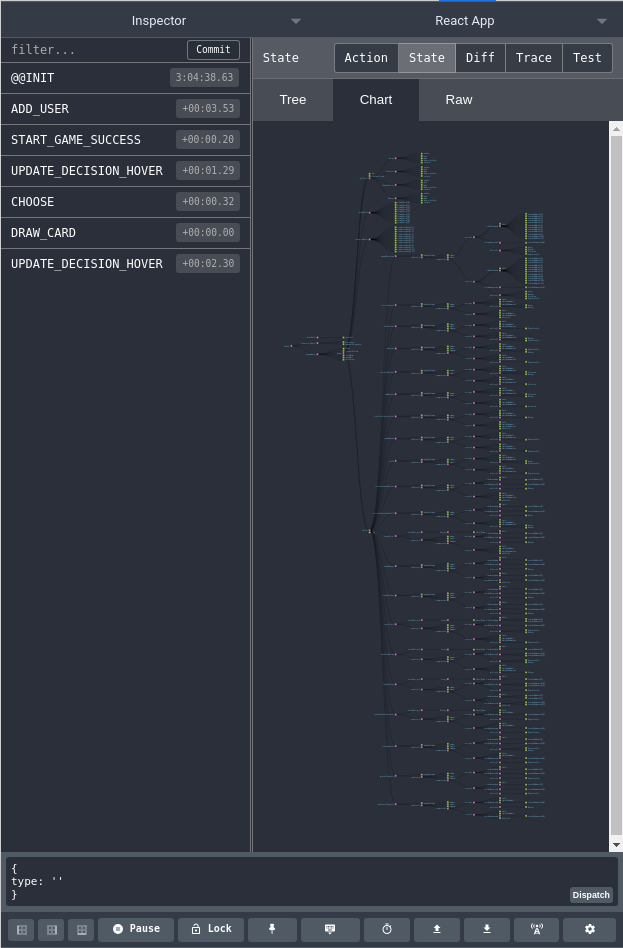
\includegraphics[width=0.8\textwidth]{./images/impl/redux_view.png}
	\caption{Redux DevTool \cite{ReduxDev} opened in game view. This shows what actions have occurred while the page has been open, as well as visualising the application state.}
	\label{fig:redux_view}
\end{figure}

\subsection{NeDB}
To store both the game definitions and the gameplay data, I needed a form of server-side persistance. I had  decide here between designing and maintaining a rigid relational database, or opting for a NoSQL \cite{NoSQL} solution. After consideration, I chose to go with a document-based database. The main factor in this decision was that I was unsure of what data would be desired by users of the final product. While a relational database requires strict definitions of data and their types, document-based databases are much more free form, meaning values can be added and removed with no alterations to the database server required.

Specifically, I chose to use NeDB\cite{NeDB}. NeDB is a lightweight JS database library that was quick and easy to set up and use. The API it provides is a subset of that of MongoDB\cite{MongoDB}, and was therefore well documented despite this being a smaller, more lightweight tool. Game definitions and user data are stored in two separate instances.

This database implementation does have some downsides in terms of long term maintenance - ideally further along in the project's life cycle this would probably be converted to a relational database, once the data requirements were more strictly defined. Also, regrettably NeDB does not expose encryption as part of its API.
This was something I only became aware of towards the end of the project, I might have chosen a different library if this had been immediately obvious. It would still be possible to encrypt fields individually
It did however suit the needs of the project, and I believe I made the right choice in getting started with NoSQL.

\section{Frontend}

\subsection{Game}

\subsubsection{Logic}
Most of the game logic happens in the redux reducers. 
This is the part of the code where actions arrive and the payload gets processed, resulting in some change to the game state which is then propagated through the page.

Reducers should technically be pure functions, as this makes them reliably testable and allows the time travel aspect of the debug tools to work correctly. 
I have followed this convention for all of my reducers, except for \c{CHOOSE}, which is called when the player makes a choice. 
This is because of the shuffle function that gets called, which has a random element.

The shuffle function I used is an implementation of the Fisher-Yates Shuffle\cite{Shuffle}. 
I needed this to ensure that the game remained unpredictable across replays, improving replayability.

Building the play deck is simply a case of iterating through each card that is out of play and adding those that match the requirements, as well as iterating through the previous play deck and removing those that do not.

\subsubsection{Images}
The colouring of images was one of the more technically involved parts of the project. 
In order to avoid heavily pixel processing I knew I would have to use SVGs, which can be edited with comparably insignificant computation (also having the advantage of being infinitely scalable). 
I then had to acquire some example images to use for my game definition. 
To maintain a similar art style I sourced them all from the same artist, Katerina Limpitsouni, on her site unDraw\cite{Undraw}. These images are open-source and usable for free and without attribution. 
The website has the advantage of allowing the main colour of each image downloaded to be set through a colour picker. 
After failing to find a solution to edit specific colours of an SVG in JavaScript, I resorted to wrapping each image in a React component, which passes through and injects the desired colour. 
This was not a favourable solution, as it's not possible to do this through the game maker tool. 
Considering this a prototypical feature (and not part of requirements), I believe the implementation is satisfactory.

Alternatively to this solution, another, less technically challenging but more time consuming possibility would be to fill the image URL property of each card, which could then be downloaded and rendered client-side.

\subsubsection{Hover}
When the user hovers over an answer with the mouse, the pillars affected by that response are outlined with a border, the colour of which depends on whether the effect is positive or negative. 
There were multiple ways in which this could have been implemented; I decided to use an enum property in the global state. 
Doing so makes it extensible - other effects or other hovering elements could be added easily.

\subsection{Game Maker}
Much of the time I spent working with CSS was on the game maker page, particularly the card and pillar views. 

Within the cards, if any text overflows beyond the limit of its section, it slowly fades out towards the bottom. This indicates to the user that there is more text to read, avoiding the situation where text is cut off but this is disguised by the gap between two lines of text. This effect is achieved by adding a fixed-height, partially transparent gradient matching the background colour to the bottom of each text \c{div}.

Cards are displayed in a responsive grid, which was done using CSS-flexboxes. I first used a combination of the \c{flex-basis}, \c{min-width} and \c{max-width} properties to allow each card to expand and contract slightly beyond its initial size. These were then placed inside a \c{div} with \c{display:flex}, allowing the cards to dynamically size and arrange themselves according to the size of this parent container. Using the Emotion\cite{Emotion} library, I was able to inject inline styles into the \c{hover} attribute of the card component, which allowed me to create the card expansion effect on hovering over them. The responseive nature of the site can be seen in figure \ref{fig:responsive}.

\begin{figure}[!h]
	\centering
	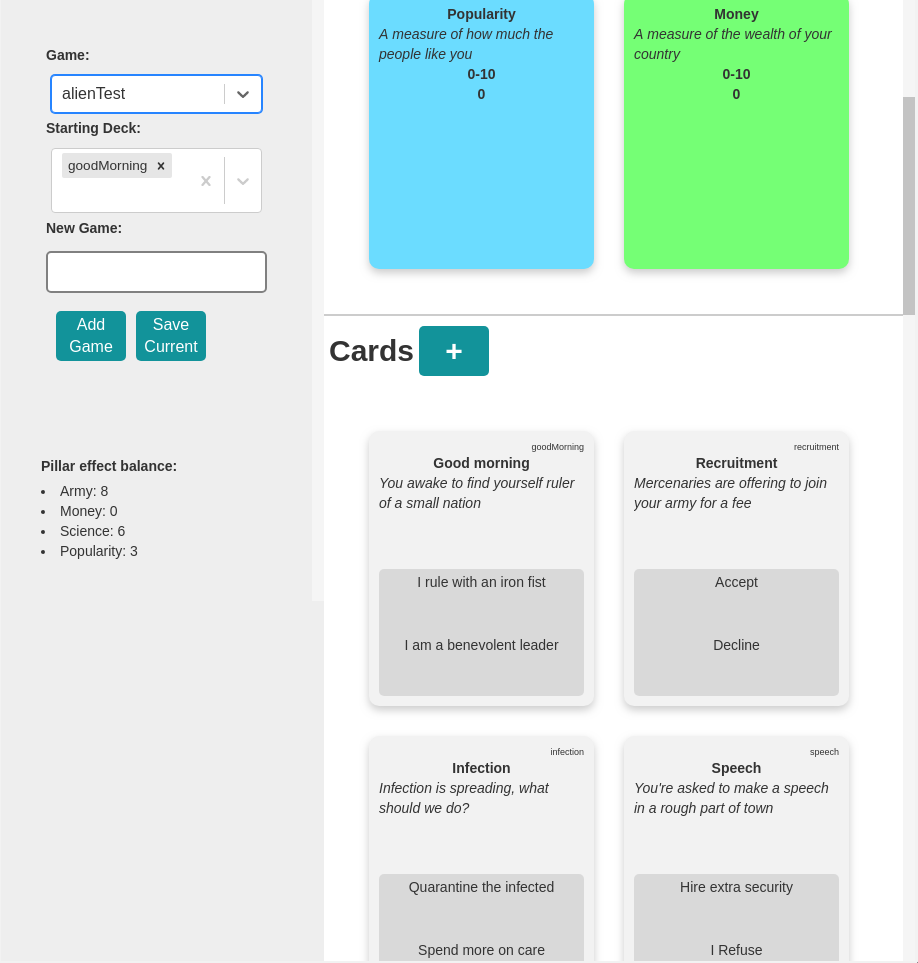
\includegraphics[width=0.8\textwidth]{./images/impl/responsive.png}
	\caption{Game maker at 960x1080 - note that all infomation is still visible.}
	\label{fig:responsive}
\end{figure}

\section{Testing}
Thanks to the structure enforced by Redux, the application logic is entirely contained within one file - \c{reducers.tsx}. This simplifies testing, as the important code can be covered with a few well chosen unit tests. To write these tests I used Jest\cite{Jest} - a fairly simple JavaScript testing framework.